\section{การเรียนรู้เชิงลึก (Deep Learning)}
การเรียนรู้เชิงลึก (Deep Learning) คือความพยายามในการจำลองเซลล์ประสามของมนุษย์ให้อยู่ในรูปโมเดลคณิตศาสตร์
ด้วยความเชื่อทางหลักประสาทวิทยา (neurosciences) ว่าความฉลาดของสมองมนุษย์เกิดขึ้นได้จากโครงข่ายประสาทจำนวนมาก
ที่เชื่อมเข้าถึงกัน

\subsection{เปอร์เซปตรอน (Perceptron)}
\begin{figure}[h]
    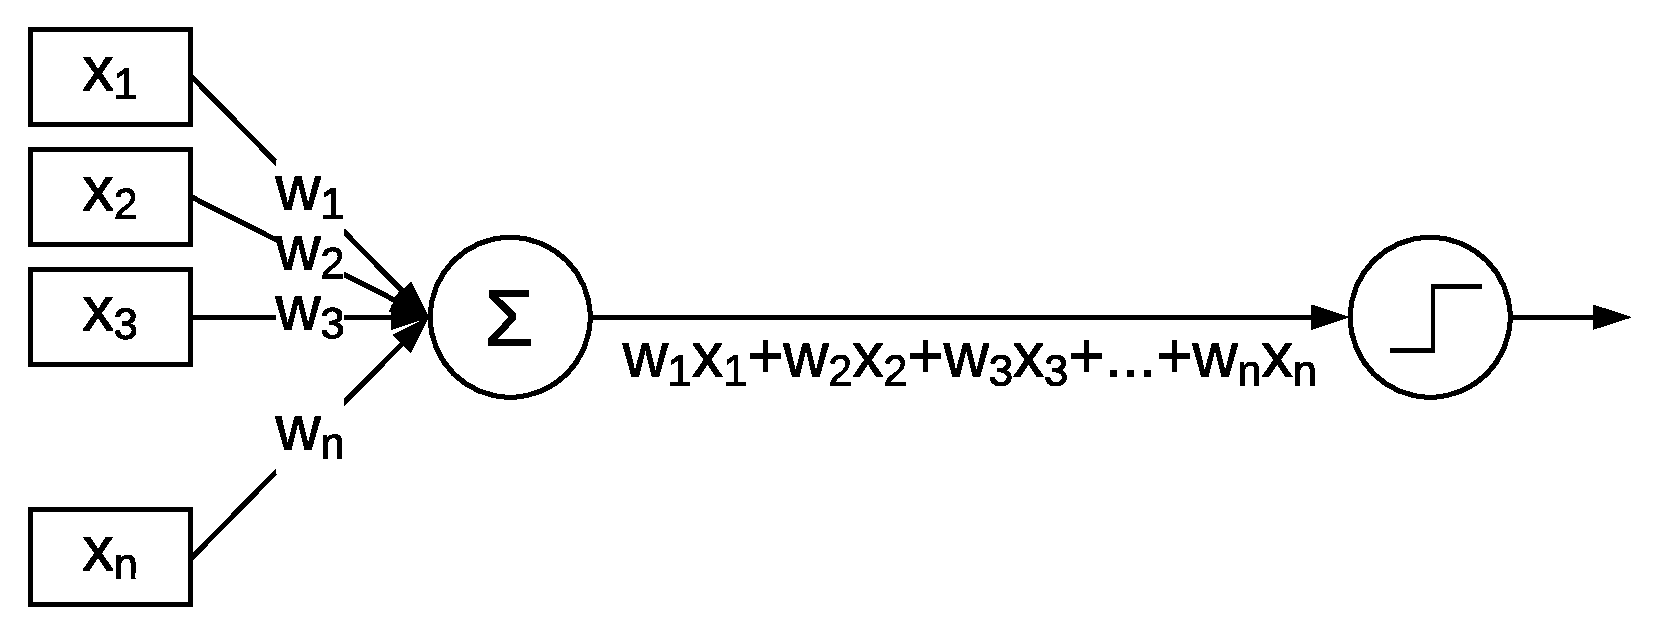
\includegraphics[width=\textwidth]{images/perceptron.pdf}
    \caption{เปอร์เซปตรอน}
\end{figure}
เปอร์เซปตรอน (Perceptron) เป็นแบบจำลองทางคณิตศาสตร์ของเซลล์สมองหนึ่งเซลล์ โดยมีคุณสมบัติดังนี้

\begin{itemize}
    \item รับเข้าข้อมูลมาในเซลล์จากหลายแหล่ง และให้น้ำหนักกับข้อมูลนั้นต่างกันไป
    \item ส่งออกข้อมูลเพียงค่าเดียว
\end{itemize}

ดังนั้น แบบจำลองทางคณิตศาสตร์สามารถเขียนออกมาจากหลักการสองข้อดังกล่าวได้ด้วยสมการ

$$ y = f\left(W^TX+b\right) $$

เมื่อ $W$ และ $X$ เป็นเวกเตอร์ขนาด $1 \times n$ (โดย $n$ เป็นจำนวนข้อมูลรับเข้า), $b$ เป็นค่าสัมประสิทธิ์คงที่ (ไบแอส: bias)
และ $f$ เป็นฟังก์ชั่นกระตุ้น (activation function)

ยกตัวอย่างการใช้เปอร์เซปตรอนในการแก้ปัญหาอย่างง่ายได้ในที่นี้

\subsubsection{การคาดเดาราคาอสังหาริมทรัพย์}
หากสำรวจราคาอสังหาริมทรัพย์แล้วพบว่า
\begin{itemize}
    \item ราคาอสังหาริมทรัพย์จะเพิ่มขึ้นตามที่ดิน โดยเพิ่มขึ้นทุก 10,000 บาทต่อตารางวา
    \item ราคาอสังหาริมทรัพย์จะเพิ่มขึ้นตามจำนวนห้องนอน โดยเพิ่มขึ้นทุก 200,000 บาทต่อห้องนอน
    \item ราคาอสังหาริมทรัพย์จะลดลงตามจำนวนอายุปี โดยลดลงทุก 7,000 บาทต่ออายุของอสังหาริมทัพย์
\end{itemize}
\noindent
จะสามารถเขียนเปอร์เซปตรอนเพื่อคาดเดาราคาอสังหาริมทรัพย์ได้โดย
$$ y = f\left(W^TX+b\right) $$
เมื่อ $W$ ซึ่งเป็นค่าสัมประสิทธิ์แสดงถึงความสัมพันธ์ข้อมูลรับเข้า ซึ่งเขียนได้จากความสัมพันธ์ดังแสดงด้านล่าง
$$
    W^T = \begin{bmatrix}
        10000 & 200000 & -7000
    \end{bmatrix}
$$
$b$ เป็นไบแอส, จะสมมติให้ $b = 500000$ (ราคาตั้งต้นของบ้าน 0 ห้องนอน พื้นที่ 0 ตารางวา อายุ 0 ปี) 
และ $f(x) = x$ กล่าวคือเป็นฟังก์ชั่นเชิงเส้น

หากต้องการคาดเดาราคาบ้านที่มี 3 ห้องนอน เนื้อที่ 100 ตารางวา และมีอายุ 7 ปี จะสามารถเขียนเวกเตอร์ $P$ ได้เป็น

$$
    X = \begin{bmatrix}
        3 \\
        100 \\
        7
    \end{bmatrix}
$$
และผลการทำนายราคาบ้านคำนวนได้จาก
$$
    \begin{aligned}
        y &= f\left(W^TX+b\right)\\
        &= f\left(\begin{bmatrix}
            10000 & 200000 & -7000
        \end{bmatrix} \times \begin{bmatrix}
            3 \\
            100 \\
            7
        \end{bmatrix}\right)\\
        &= f(30000 + 20000000 + (-49000)) = f(19981000)\\
        &= 19981000
    \end{aligned}
$$

\subsubsection{การสร้างประตูสัญญาณตรรกะด้วยเปอร์เซปตรอน}
เราสามารถสร้างประตูสัญญาณตรรกะ (logic gates) บางชนิดได้ด้วยเปอร์เซปตรอน เช่นการสร้าง AND และ OR gate

ยกตัวอย่างโครงสร้างของ AND gate ซึ่งสามารถสร้างได้ด้วยการกำหนดให้
\begin{itemize}
    \item $X$ เป็นเมทริกซ์ขนาด $1 \times 2$ กล่าวคือเมื่อรับค่า $x_1, x_2$ เป็นค่า 0 หรือ 1 แทนสัญญาณจริงหรือเท็จแล้ว
        $$X = \begin{bmatrix}
            a_1 \\
            a_2
        \end{bmatrix}$$
    \item กำหนดค่าของเมทริกซ์ $W$ เป็น
        $$W^T = \begin{bmatrix}
            1 && 1
        \end{bmatrix}$$
    \item กำหนดค่าของไบแอส $b = -2$
    \item กำหนดฟังก์ชั่น $f(x)$ เป็น step function กล่าวคือ
    $$ f(x) = 
    \begin{cases} 
        0 & \textrm{เมื่อ } x < 0 \\
        1 & \textrm{เมื่อ } x\geq 0
    \end{cases}
    $$
\end{itemize}
และการสร้าง OR gate สามารถทำได้ในลักษณะเดียวกันโดยเปลี่ยน $b$ เป็น $b = -1$

\subsection{เปอร์เซปตรอนแบบหลายชั้น (Multi Layer Perceptron)}

เราอาจสังเกตว่าเปอร์เซพตรอนหนึ่งตัวนั้นทำหน้าที่ได้เพียนแยก (classify) หรือถดถอย (regress) ปัญหาที่เป็นปัญหาเชิงเส้น (linear problems) ได้เท่านั้น อย่างไนก็ตามหากเรากำหนดให้ฟังก์ชั่น $f$ เป็นฟังก์ชั่นที่ไม่ใช่ฟังก์ชั่นเส้นตรงแล้ว เราอาจสร้าง\textbf{เปอร์เซปตรอนแบบหลายชั้น} (Multi Layer Perceptron) ขึ้นมาได้โดยมีลักษณะดังนี้